\section{Issue Tracking System}

\begin{mdframed}
    \textbf{Issue Tracking System}: computer software package that manages and maintains lists of issues, as needed by an organization.
\end{mdframed}
\begin{itemize}
    \item \textbf{Issue:} criticità, attività/evento da gestire
    \item \textbf{Tracking:} registrare, lasciare delle tracce
\end{itemize}

\subsection{Utilizzo}
\begin{itemize}
    \item \textbf{Condividere} le informazioni
    \begin{itemize}
        \item unica repository dove trovare le informazioni
        \item sistema di notifica
        \item dashboard
    \end{itemize}
    \item Implementare un processo per misurarne la \textbf{qualità}
    \item Avere un'istantanea dello \textbf{stato del progetto}
    \begin{itemize}
        \item attività da fare
        \item in corso d'opera
        \item completate
    \end{itemize}
    \item Decidere quando e cosa \textbf{rilasciare}
    \item Assegnare e dare \textbf{priorità alle attività}
    \item Consultare il \textbf{tempo impiegato}
    \item Avere una chiare \textbf{assegnazione delle attività}
    \item \textbf{Memoria storica} di tutti i cambiamenti del progetto
\end{itemize}

\subsection{Work Item}
\begin{mdframed}
    \textbf{Work item:} singola attività minima del progetto, gestita mediante un workflow e mantenuta all'interno di un'unica piattaforma e di un'unica repository.
\end{mdframed}

\subsubsection{Caratteristiche}
\begin{itemize}
    \item \textbf{Progetto:} progetto a cui si riferisce
    \item \textbf{ID:} identificativo univoco
    \item \textbf{Descrizione:} descrizione dell'attività
    \item \textbf{Tipo:} categoria del work item
    \item \textbf{Stato:} stato all'interno del workflow in cui si trova il work item
    \item \textbf{Priorità:} importanza del work item in relazione con gli altri work item del progetto
    \item \textbf{Tag:} permettono di classificare i work item, anche di diversi tipi
    \item \textbf{Collegamenti:} permettono di collegare tra loro i work item
    \item \textbf{Assegnatario:} identifica chi è il responsabile per svolgere l'attività
    \item \textbf{Segnalante:} identifica chi ha segnalato l'attività
    \item \textbf{Data:} data di creazione, di ultimo aggiornamento, di risoluzione
    \item \textbf{Allegati:} file allegati
\end{itemize}

\subsection{Workflow}
\begin{mdframed}
    \textbf{Workflow:} insieme di stati e transizioni che un Work Item attraversa durante il suo ciclo di vita.
\end{mdframed}
\begin{itemize}
    \item Permette di implementare il processo da seguire per completare l'attività
    \item Viene associato ad un progetto e può essere associato a uno o più tipi
    \item Permette di registrare tutte le transizioni e cambi si stato
\end{itemize}
\begin{center}
    \begin{tabular}{c}
        \\ 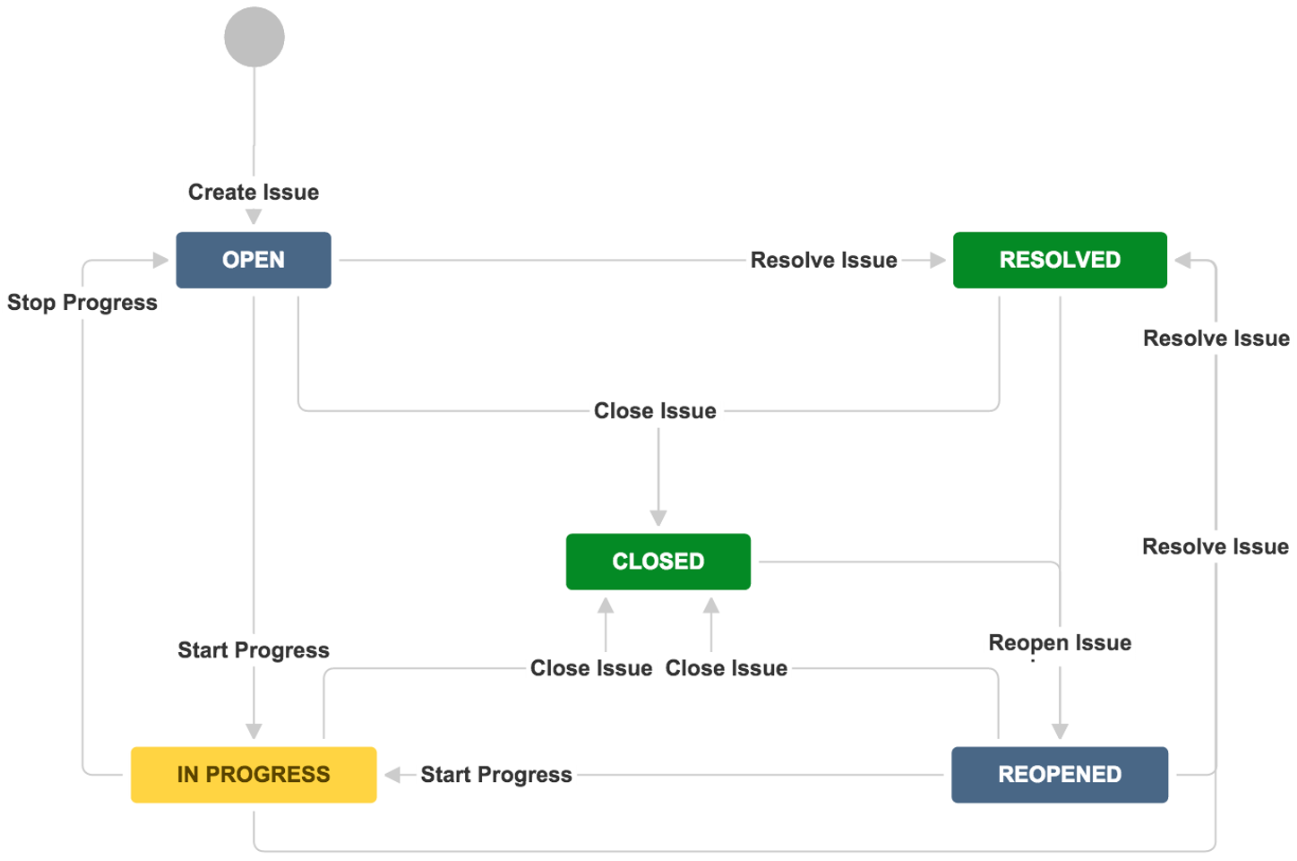
\includegraphics[width=0.9\textwidth]{images/ITS1.png} \\ \\
    \end{tabular}
\end{center}

\subsection{Funzionalità}
\begin{multicols}{3}
    \raggedright
    \textbf{Gestione:}
    \begin{itemize}
        \item Ricerca avanzata dei work item
        \item Salvataggio di ricerche
        \item Esportazione
        \item Reporting
    \end{itemize}
    \columnbreak
    \textbf{Integrazione:}
    \begin{itemize}
        \item Integrazione con il Source Code Management
        \item Integrazione con l'ambiente di sviluppo
        \item[]
        \item[]
    \end{itemize}
    \columnbreak
    \textbf{Condivisione:}
    \begin{itemize}
        \item Notifiche
        \item Bacheche o Board
        \item Dashboard
        \item Definizione di Road Map e Release Notes
    \end{itemize}
\end{multicols}

\subsubsection{Filtri}
\begin{itemize}
    \item Ricercare i work item in base ai campi
    \item Salvati per facilitare le ricerche più frequenti
    \item Risultati possono essere esportati
    \item Base per creare report, board e dashboard
\end{itemize}

\subsubsection{Board}
\begin{itemize}
    \item Visualizzare i work item di uno o più progetti, offrendo in modo flessibile e iterativo di visualizzazione, gestione e visualizzare dati di sintesi sulle attività in corso
    \item Configurare e visualizzare i work item ricercati con un filtro
    \item Interagire velocemente con i work item
\end{itemize}

\subsubsection{Report}
\begin{itemize}
    \item Monitorare e avere una visione d'insieme del progetto
\end{itemize}

\subsection{Configurazione}
\begin{center}
    \begin{tabular}{c}
        \\ 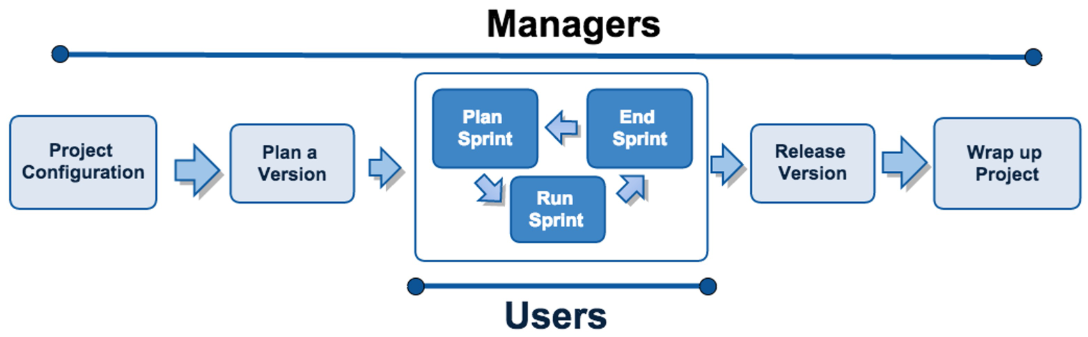
\includegraphics[width=0.9\textwidth]{images/ITS2.png} \\ \\
    \end{tabular}
\end{center}

\subsubsection{Obiettivi}
\begin{itemize}
    \item Identificare i processi richiesti per la gestione del progetto:
    \begin{itemize}
        \item Procedure e best practices definiti dai framework di qualità presenti in azienda o richiesti dal cliente
        \item Vincoli imposti dal cliente
        \item Modalità di gestione del progetto del team
    \end{itemize}
    \item Identificare e configurare gli strumenti che permettono di implementare i processi:
    \begin{itemize}
        \item Identificazione e definizione dei tipi, campi custom, workflow e collegamenti che ci permettono di tracciare le informazioni richieste dal processo
    \end{itemize}
\end{itemize}

\subsubsection{Configurazine}
\begin{multicols}{2}
    \raggedright
    \textbf{Admin:}
    \begin{itemize}
        \item Crea un nuovo progetto
        \item Definisce il processo da seguire:
        \begin{itemize}
            \item tipi di work item, campi custom, workflow, collegamenti
            \item seleziona il modello di stima
            \item board e report per processo
        \end{itemize}
        \item Aggiunge gli utenti e assegna ruoli/permessi
    \end{itemize}
    \columnbreak
    \textbf{Capo progetto:}
    \begin{itemize}
        \item Definisce le versioni [release]
        \item Definisce le componenti del progetto
        \item Definisce il lavoro da svolgere [backlog]:
        \begin{itemize}
            \item priorità
            \item assegnatario
            \item stima
        \end{itemize}
        \item Definisce la prima iterazione
    \end{itemize}
\end{multicols}

\subsubsection{Utilizzo}
\begin{multicols}{2}
    \raggedright
    \textbf{Team di Sviluppo:}
    \begin{itemize}
        \item Riceve le notifiche dei work item assegnati
        \item Selezionano i work item in base alle priorità
        \item Avviano e completano la lavorazione:
        \begin{itemize}
            \item avanzano gli stati del workflow
            \item aggiornano la stima a finire
            \item registrano il tempo impiegato
        \end{itemize} 
        \item Documentano lo stato dell'attività (commenti) e compilano e campi nel work item
        \item Completano tutte le attività presenti nell'iterazione
        \item Effettuano il rilascio
    \end{itemize}
    \columnbreak
    \textbf{Capo progetto:}
    \begin{itemize}
        \item Monitora l'avanzamento e il completamento delle attività (filtri, board. dashboard, report)
        \item Definisce le nuove versioni
        \item Definisce le nuove iterazioni
        \item Definisce, aggiorna e monitora le attività (priorità, verifica stima)
        \item Produce i report richiesti dal cliente
        \item[]
    \end{itemize}
\end{multicols}

\newpage